\documentclass[conference]{IEEEtran}
%\usepackage{graphicx}
\usepackage[dvipdfmx]{graphicx}
%\usepackage{latexsym}
\usepackage{slashbox}
%\usepackage{multirow}
\usepackage{url}
\usepackage{color}
\usepackage{colortbl}
\usepackage{hhline}
\usepackage{flushend}
\usepackage{verbatim}
%\usepackage{hyperref}
\usepackage{enumerate}
\usepackage[sort&compress]{natbib}
\usepackage{subfigure}
\usepackage{framed}
%\usepackage{natbib}

\newcommand{\todo}[1]{{\color{green}{\textbf{TODO: [#1]}}}}
\newcommand{\yasu}[1]{{\color{red}{\textbf{Yasu says: [#1]}}}}
\newcommand{\emad}[1]{{\color{blue}{\textbf{[#1]}}}}
\newcommand{\Emad}[1]{{\color{blue}{\textbf{[#1]}}}}
\newcommand{\revised}[1]{{\color{red}{#1}}}
\newcommand{\para}[1]{{\color{magenta}{\textbf{This paragraph:}}} [#1]}

%\newcommand{\revised}[2]{\marginpar{\fbox{#2}}{\color{red}{#1}}}

\newcommand{\nbf}[1]{
%  \noindent{\textit{\textbf{#1}}}
  \noindent{\textbf{#1}}
}

\newcommand{\conclusionbox}[1]{%
	\vspace{2mm}
  \noindent
	\framebox[0.48\textwidth][c]{%
		\parbox[b]{0.45\textwidth}{%
			{\em #1}
		}
	}
}

% Set bibliography title
%\renewcommand\refname{REFERENCES}
%\renewcommand\bibsection{\section{\refname}}

\newcommand{\ea}{{\em et al.}}
\newcommand{\smallsection}[1]{\vspace{1mm}\noindent {\bf #1}.\hspace{2mm}}
\newcommand{\emphsection}[1]{\vspace{1mm}\noindent \underline{{\em #1}.}\hspace{2mm}}


% Reduce bibliography font size
%\def\bibfont{\normalsize} %normalsize should be default
% small or footnotesize

% Reduce space between references
%\setlength{\bibsep}{3.2pt} %3.5pt should be default


\begin{document}

\title{Using Analytics to Quantify Interest of Self-Admitted Technical Debt}

\author{
\IEEEauthorblockN{Yasutaka Kamei$^{\dag}$, Everton Maldonado$^{\dag\dag}$, Emad Shihab$^{\dag\dag}$, and Naoyasu Ubayashi$^{\dag}$}
\IEEEauthorblockA{
$^{\dag}$Principles of Software Languages Group (POSL), Kyushu University, Fukuoka, Japan\\
$^{\dag\dag}$Department of Computer Science and Software Engineering, Concordia University, Montr\'eal, Canada\\
Email: $^{\dag}$\{kamei, ubayashi\}@ait.kyushu-u.ac.jp, $^{\dag\dag}$\{e\_silvam, eshihab\}@encs.concordia.ca
}
}

% make the title area
\maketitle

% As a general rule, do not put math, special symbols or citations
% in the abstract
\begin{abstract}
Technical debt refers to the phenomena of taking a shortcut to achieve short term development gain at the cost of increased maintenance effort in the future. The concept of debt, in particular, the cost of debt has not been widely studied. Therefore, the goal of this paper is to determine ways to measure the `interest' on the debt and use these measures to see how much of the technical debt incurs positive interest, i.e., debt that indeed costs more to pay off in the future. To measure interest, we use the LOC and Fan-In measures. We perform a case study on the Apache JMeter project and find that approximately 42 - 44\% of the technical debt incurs positive interest.
%do we know how much interest we are paying on the technical debt in software development projects?
%To tackle this problem, we aim to quntify interest of Self-Admitted Technical Debt (SATD) using analytics
%such as software metrics and automatic SATD detection techniques. We conduct an initial case study using the dataset collected
%from the Apache JMeter projet. The results show that 44.2\% of technical debt has a positive rate in terms of LOC and 42.2\% of technical debt has it in terms of Fan-In.
\end{abstract}

\IEEEpeerreviewmaketitle

% Here is Yasu't note
\begin{comment}
2 tomato: let's finish results (how to show)
2 tomato: read related work to get knowledge and good motivation for RQ1 and RQ2.

- slide:
2 tomato (one topic of current)
2 tomato (one topic of current)
\end{comment}

%%%%%%%%%%%%%%%%%%%%%%%%%%%%%%%%%%%%%%%%%%%%%%%%%%%%%%%%%%%
%%What is technical debt and self-admitted technical debt
Technical debt is term first coined by Cunningham in 1993 to refer to the phenomena of taking a shortcut to achieve short term development gain at the the cost of increased maintenance effort in the future \cite{Cunningham1992WPM}. The technical debt community, organized through the managing technical debt workshop \cite{Falessi2014MTD}, has studied many aspects of technical debt, including its detection \cite{Zazworka2013CSE}, impact \cite{Zazworka2011MTD}
and the appearance of technical debt in the form of code smells \cite{Fontana2012MTD}. Most recently, we developed an approach to identify technical debt from code comments, referred to as self-admitted technical debt (SATD). SATD refers to the situation where developers know that the current implementation is not optimal and write comments alerting the inadequacy of the solution.

% What people did and what is the impact of TD. What they found.
In the last few years, an increasing amount of work has focused on SATD. In particular, our prior work focused on the detection of SATD~\cite{Potdar2014ICSME} and the classification of different types of SATD and the development of datasets to enable future studies on SATD~\cite{Maldonado2015MTD}. Other work by Bavota and Russo performed an empirical study of SATD on a large number of Apache projects showed that SATD is prevalent in open source projects, is long lived and is increasing over time. A study by Wehaibi et al. \todo{cite Wehaibi} examined the impact of SATD on quality and found that SATD does not necessarily relate to more defects, however, it does make the software system more complex. 

%However, very little work focused on interest. Also, why is calculating interest difficult
Based on these prior findings, we measure and quantify the effect of SATD. In particular, we measure the amount of \emph{interest} caused by SATD. Although the metaphor of technical debt has been well studied, to the best of our knowledge, the quanitification of interest of technical debt has not been examined before. Measuring the interest if technical debt is non-trivial since it requires, in addition to the detection of the technical debt, the tracking of the debt over time and the development of a measure to accurately quantify this debt.

% What we do  and how we calculate interest
In this paper, we first propose the use of code metrics, in particular \todo{add}, as a measure of interest. We 
 
% Main contributions
The main contributions of the paper are three-fold.

\begin{itemize}
\end{itemize}

% Organization of the paper
\smallsection{Paper Organization} To purse the goal of this paper, the paper is organized as follows. 
Section \ref{background} explains the overview of defect prediction models.
Section \ref{past} revisits what challenges were in Year 2000.
%Section \ref{trends} assesses what state the research trend is in.
%Section \ref{game_changers} presents game changers, which dramatically changed perspective and direction of the studies in the field of defect prediction.
Section \ref{trends} assesses what state the research trend is in and presents some of game changers, which dramatically changed perspective and direction of the studies in the field of defect prediction.
Section \ref{challenges} highlights some key challenges for future.
Section \ref{conclusion} draws conclusions.


%\section{Introduction}
%What is technical debt and self-admitted technical debt
Technical debt is term first coined by Cunningham in 1993 to refer to the phenomena of taking a shortcut to achieve short term development gain at the the cost of increased maintenance effort in the future \cite{Cunningham1992WPM}. The technical debt community, organized through the managing technical debt workshop \cite{Falessi2014MTD}, has studied many aspects of technical debt, including its detection \cite{Zazworka2013CSE}, impact \cite{Zazworka2011MTD}
and the appearance of technical debt in the form of code smells \cite{Fontana2012MTD}. Most recently, we developed an approach to identify technical debt from code comments, referred to as self-admitted technical debt (SATD). SATD refers to the situation where developers know that the current implementation is not optimal and write comments alerting the inadequacy of the solution.

% What people did and what is the impact of TD. What they found.
In the last few years, an increasing amount of work has focused on SATD. In particular, our prior work focused on the detection of SATD~\cite{Potdar2014ICSME} and the classification of different types of SATD and the development of datasets to enable future studies on SATD~\cite{Maldonado2015MTD}. Other work by Bavota and Russo performed an empirical study of SATD on a large number of Apache projects showed that SATD is prevalent in open source projects, is long lived and is increasing over time. A study by Wehaibi et al. \todo{cite Wehaibi} examined the impact of SATD on quality and found that SATD does not necessarily relate to more defects, however, it does make the software system more complex. 

%However, very little work focused on interest. Also, why is calculating interest difficult
Based on these prior findings, we measure and quantify the effect of SATD. In particular, we measure the amount of \emph{interest} caused by SATD. Although the metaphor of technical debt has been well studied, to the best of our knowledge, the quanitification of interest of technical debt has not been examined before. Measuring the interest if technical debt is non-trivial since it requires, in addition to the detection of the technical debt, the tracking of the debt over time and the development of a measure to accurately quantify this debt.

% What we do  and how we calculate interest
In this paper, we first propose the use of code metrics, in particular \todo{add}, as a measure of interest. We 
 
% Main contributions
The main contributions of the paper are three-fold.

\begin{itemize}
\end{itemize}

% Organization of the paper
\smallsection{Paper Organization} To purse the goal of this paper, the paper is organized as follows. 
Section \ref{background} explains the overview of defect prediction models.
Section \ref{past} revisits what challenges were in Year 2000.
%Section \ref{trends} assesses what state the research trend is in.
%Section \ref{game_changers} presents game changers, which dramatically changed perspective and direction of the studies in the field of defect prediction.
Section \ref{trends} assesses what state the research trend is in and presents some of game changers, which dramatically changed perspective and direction of the studies in the field of defect prediction.
Section \ref{challenges} highlights some key challenges for future.
Section \ref{conclusion} draws conclusions.


%\para{What is technical debt?}
%
%\para{Describe more detail of technical debt and current problem in the domain}
%
%\para{The goal and approach of this study}
%
%\para{Contributions}
%
%\cite{Potdar2014ICSME}
%\cite{Maldonado2015MTD}

%%%%%%%%%%%%%%%%%%%%%%%%%%%%%%%%%%%%%%%%%%%%%%%%%%%%%%%%%%%
%\section{Background} \label{background}
%\emph{Prevention is better than cure.}
\para{Technical debt}

\cite{Guo2011ICSM}: they track technical debt items and access its impact (cost) among incurred, deferred and paid. That said, they focused on only one event (WebDav protocol is not supported) and 

\para{Software Evolution: We calculate interest by looking at the difference size of two versions. In other words, this work is one of lines of software evolution.}

%%%%%%%%%%%%%%%%%%%%%%%%%%%%%%%%%%%%%%%%%%%%%%%%%%%%%%%%%%%

%-----------------------------------------------------------------------
\begin{figure*}[!t]
  \begin{center}
  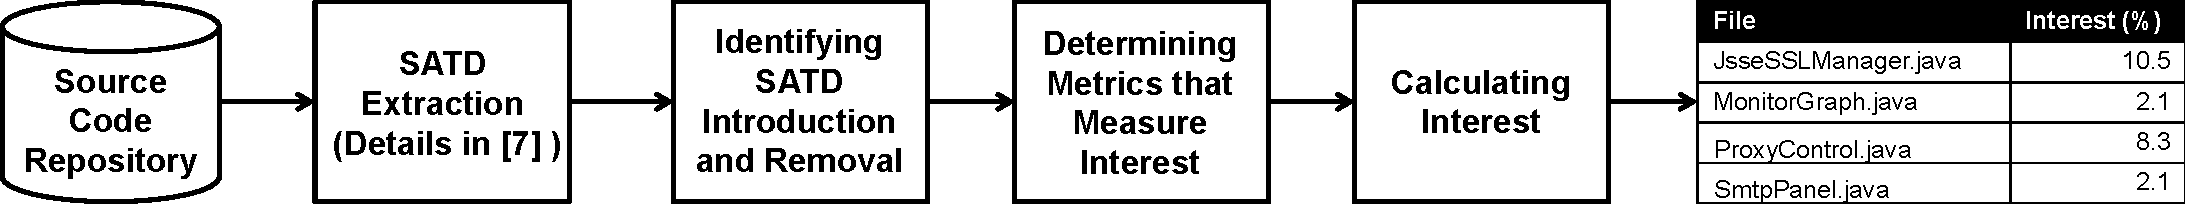
\includegraphics[width=.95\textwidth]{figures/overview}
  \caption{The overview of our approach.}
  \label{fig:overview}
  \end{center}
\end{figure*}
%-----------------------------------------------------------------------


%\section{Case Study Setup} \label{sec:setup}
\section{Approach} \label{sec:approach}
To perform our study, we need to determine the SATD in the codebase, locate when the SATD was introduced in the project and when it was later removed. Then, we use our measures of interest, i.e., LOC and Fan-In, to compare the size of the code and the amount of dependence other code had on the TD code in order to quantify interest (Figure \ref{fig:overview}).

\if0
% Yasu: We just out this part for a position paper.
\subsection{SATD Extraction}
\smallsection{(Step 1) Extract source code files}
To perform our case study, we obtain source code files from Git repositories of three projects. We selected {\sc 1.4.0}, {\sc ANT\_170}, and {\sc v2\_10} in each JRuby, Apache Ant, and Apache jmeter as versions (tags) of which we extract SATD. The versions were released at the middle of project history. Therefore, we believe that projects elapse sufficient time for obtaining technical debt for our analysis and remain time for removing it.

\smallsection{(Step 2) Parse source code files}
After obtaining source code files, we extract the comments from them. We use JDeodorant~\cite{Tsantalis2008CSMR}, which is an open-source Eclipse plug-in, to parse the source code and extract the code comments. JDeodrant uses the Eclipse AST framework to create an Abstract Syntax Tree (AST) map of the source code. The AST map contains detailed information about the project such as: the source code comments, its type (e.g., Block, Single-line, or Javadoc), the line where each one of these comments begins and finishes. We extract the aforementioned information and store all comments as the candidate of SATD.

\smallsection{(Step 3) Filter Comments}
To reduce the number of comments we manually read, we filter comments that are less likely to be classified as SATD by utilizing several heuristics, similar to previous studies~\cite{Maldonado2015MTD}.

First, we eliminate license comments from the candidate of SATD, since we found that license comments are not likely to contain SATD. License comments are commonly added before the declaration of the class. Since we know the line number that the class was declared, we can easily check for comments that are placed before that line and remove them. In order to decrease the chances of removing a SATD comment while executing this filter, we do not remove comments containing one of task-reserved words (i.e., “todo”, “fixme”, or “xxx”).

Then, we also filter Javadoc comments from the candidate of SATD, since we found that they rarely mention SATD. Based on source code comments' type provided by JDeodrant, we identify Javadoc comments. Similar to the heuristics for license comments, we do not remove Javadoc comments containing at least one of task-reserved words. To do so, we create a simple regular expression that search for the task-reserved words before removing the comment.

Then, we group consecutive single-line comments as one comment. We notice that developers sometimes make long comments, using multiple single-line comments instead of a Block comment. This characteristic can hinder the understanding of the message. When considering the case that we analyze each one of these comments independently, we may misunderstand the message because each of them would be incomplete and lose the meaning.

Finally, we filter the comments that conduct {\it comment out} source code from the candidate of SATD. While commented source code may show the code that is currently not being used or the code that was used for debugging, it may not include any developer's comments. Therefore, the commented source code is less likely to be classified as SATD. We remove commented source code using a simple regular expression that captures typical Java code structures.

Table xxx shows the number of comments that are filtered by the heuristics we used. The heuristics significantly reduces the number of comments in our dataset and helps us focus on the most applicable and insightful comments. 

\todo{add a table that shows the number of comments that are filtered by several heuristics}

\smallsection{(Step 4) Manual Classification}
To extract SATD, the xxx author manually classified all comments into SATD or not.
The xxx author who made the classification has more than 8 years of experience working in the industry as a software engineer, during this time he designed, implemented and maintained several programs using, in particular the Java programming language. He developed solid skills in object orientated programming and design patterns. We consider that these qualifications provide the necessary background to conduct the manual classification of the comments.
\fi

%\subsection{Interest Extraction} \label{subsec:interest}

\smallsection{1. SATD Extraction}
In order to measure interest of the TD, our first step is to identify where it exists. Since we focus particularly on SATD, we use code comments found in the source code. We extract and parse the source code of JMeter version 2.10. To perform the parsing, we use the {\sc JDeodorant} tool~\cite{Tsantalis2008CSMR}, which allows us to extract a comment and map it to its corresponding method. Then, we apply a series of filters to remove irrelevant comments, e.g., copyright-related comments. Finally, the 2nd author\footnote{The 2nd author who made the classification has more than 8 years of experience working in the industry as a software engineer, during this time he designed, implemented and maintained several programs using, in particular the Java programming language.} manually classified all comments to determine if they are SATD comments or not and mapped these comments to their respective methods. In this study, we assume that SATD exists in the method where the comment is identified. Details regarding the dataset and the filtering applied can be found in our earlier work~\cite{Maldonado2015MTD}.


%To extract SATD, we extract source code files for a version control system. Then we extract the comments from them using JDeodorant~\cite{Tsantalis2008CSMR}, which is an open-source Eclipse plug-in, to parse the source code and extract the code comments.
%To reduce the number of comments we manually read, we filter comments that are less likely to be classified as SATD by utilizing several heuristics, similar to previous studies~\cite{Maldonado2015MTD}. Finally, the 2nd author\footnote{The 2nd author who made the classification has more than 8 years of experience working in the industry as a software engineer, during this time he designed, implemented and maintained several programs using, in particular the Java programming language.} manually classified all comments into SATD or not. See the details of the Step 1 in Maldonado and Shihab's study~\cite{Maldonado2015MTD}.


% \todo{We need to ask Everton about git commonds to find where it was introduced and removed.
\smallsection{2. Identifying SATD Introduction and Removal}
Since we are interested in measuring the interest, we need to determine the `change' over time in these SATD methods. For each of the SATD comments identified by us, we use several git commands (e.g., {\tt git log -- <PATH\_TO\_FILE>} and {\tt git cat-file <SHA1>:<PATH\_TO\_FILE>}), to trace a comment back to the commit where it was introduced. We perform this task by replaying the history commit-by-commit. Using the same technique, we are also able to detect the removal of SATD. We detect the removal of SATD when we find that the commit is removed or changed. 
%@Yasu (from Emad's call) we extract all files in versions, and check whether or not SATD is included from the first version of each file to know SATD introduction. Similar to this, we check whether or not SATD is excluded to know SATD removal. 

%@Yasu I commented out the following sentenses since they are almost similar with the above sentenses
%By tracing the comments including SATD across versions in Git repositories, we identify two versions that introduce and remove them. To trace the comments, we obtain patches between two versions over all versions for each file that includes technical debt. Then, we check each patch about whether or not technical debt is introduced and removed. \todo{Need to merge the prior 2 sentences}

\smallsection{3. Determining Metrics that Measure Interest}
Once we are able to determine the SATD comments and their associated methods, we would like to calculate the interest that is incurred over time (i.e., from the introduction of the technical debt to its removal). To do so, we extracted 16 code metrics using the {\sc Understand Tool}~\cite{Understand}. In particular, we selected all method-level complexity and size metrics that Understand is able to provide.

The reasons that we focused on complexity and size metrics are: 1) our intuition tells us that if a piece of code is introduced and then becomes more complex, then that is a good proxy for it being more difficult to deal with in the future, i.e., it incurred interest; and 2) prior work has shown that size metrics are typically highly correlated with complexity metrics, hence, we figured using size metrics (if they are highly correlated with complexity metrics in our case) would be an easier alternative to using complexity metrics.

We measured the Spearman correlation between the complexity and size metrics and found that indeed all metrics except Fan-In are highly correlated with LOC. Therefore, we decided to use the LOC metric as a measure of interest. In addition, since Fan-In is an indicator of how much a method is depended on, we decided to also include the Fan-In metric when calculating interest. The intuition being that if a method is depended on lightly when the SATD is introduced and then has many more dependencies in the future, then dealing with this SATD is much more difficult (since many dependencies may be affected). In the end, we settled on using the two metrics, LOC and Fan-In, as measures of interest.

%To calculate interest, we measure product metrics from two versions detected in Step 2 using {\sc Understand}~\cite{Understand}. We choose all metrics (e.g., LOC and Cyclymatic Complexity) that are available at the method-level in {\sc Understand}.

\smallsection{4. Calculating Interest}
Using our metrics, we consider the relative LOC and Fan-In values between the introduced and removed versions as interest. We calculate the interest per SATD instance. For example, if arbitrary metric values in the introduced and removed versions are 10 and 20 in the method where the SATD exists, the relative size is 100 (i.e, $100* \frac{(20-10)}{10}$). In cases where the SATD is not yet removed, we use the numbers from the latest version of JMeter. Our assumption here is that if the SATD incurs positive interest, then it will be more difficult to remove in the future, e.g., if the code becomes more complex compared to when the debt was taken, then it will be more difficult to deal with.

While the paper tackles the research topic that accelerates a new research direction (i.e., quantifying interest of SATD), it also has the weakness of our current approach. We elaborate on the weakness of our current approach in Section \ref{conclusion}.


\begin{figure*}[!t]
  \begin{center}
  \scalebox{0.95}{
  \begin{tabular}{cc}
    \subfigure[JMeter (LOC)]{ 
      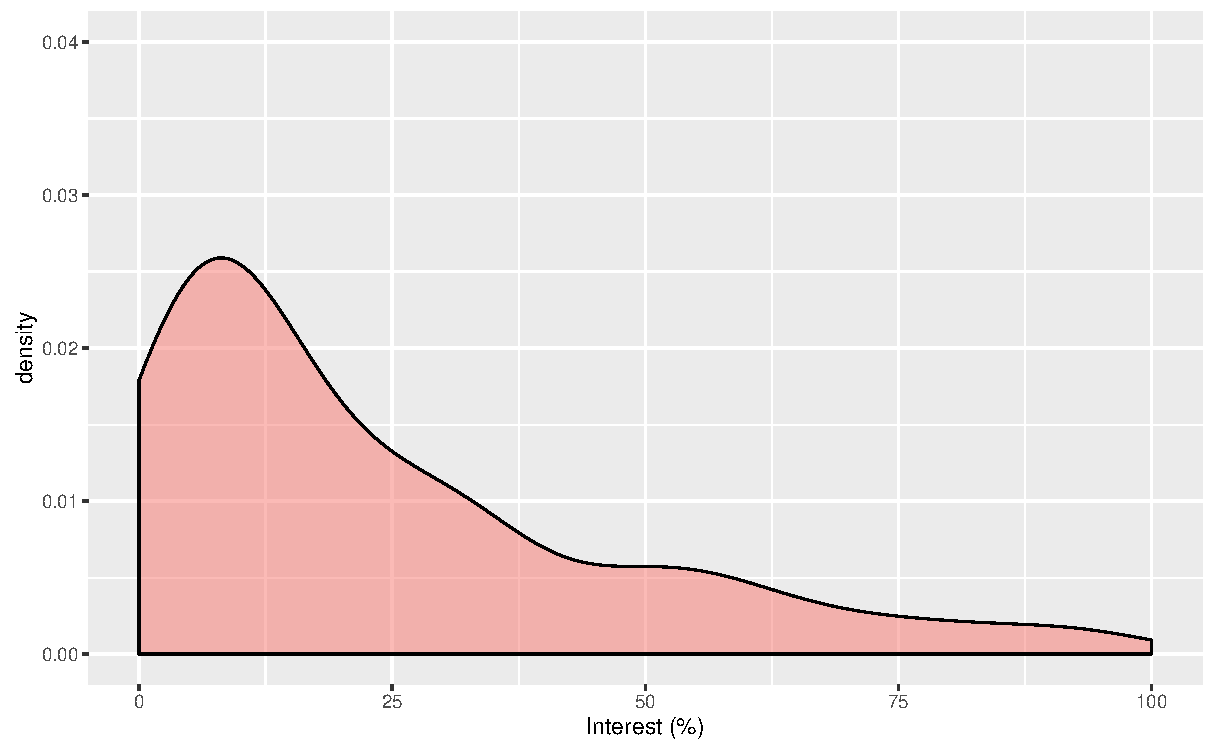
\includegraphics[width=.45\textwidth]{figures/rq1-jmeter}
    }
    \subfigure[JMeter (Fan-In)]{ 
      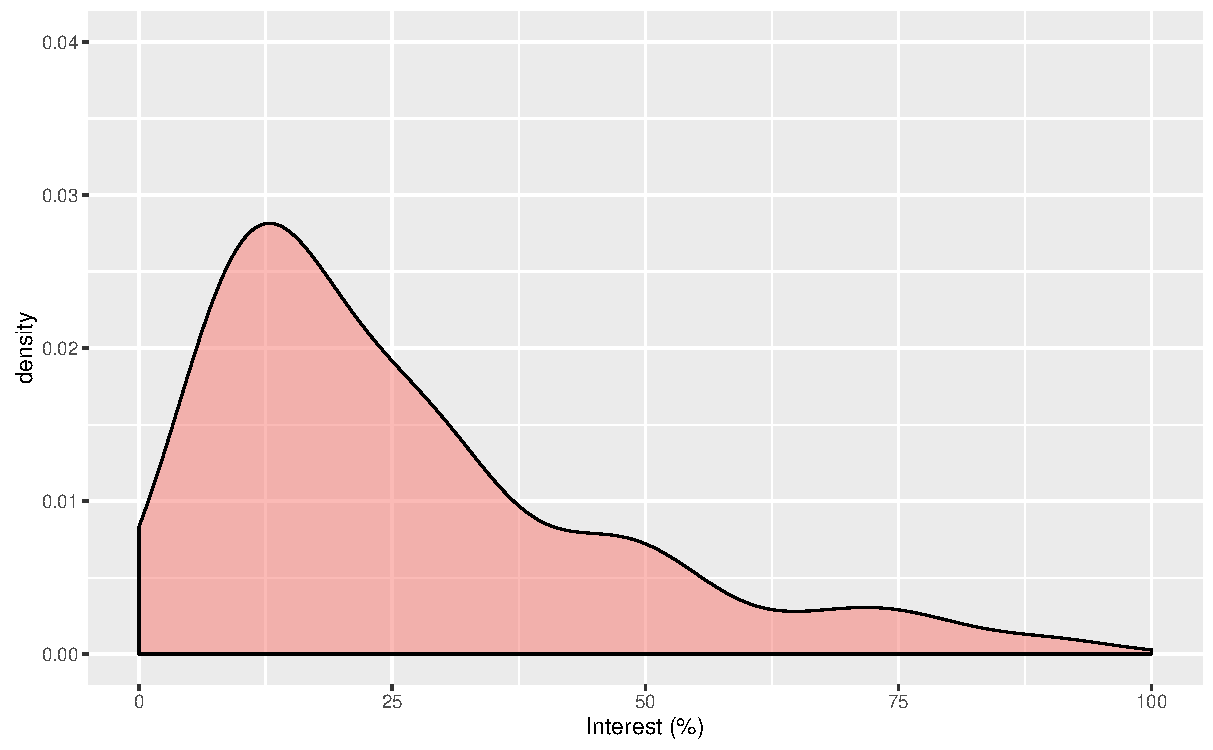
\includegraphics[width=.45\textwidth]{figures/rq1-jmeter-fanin}
    }
  \end{tabular}
  }

  \caption{Distribution of SATD Interest in JMeter. Interest is Measured Using LOC and Fan-In.}
  \label{fig:dist}
  \end{center}
\end{figure*}


%%%%%%%%%%%%%%%%%%%%%%%%%%%%%%%%%%%%%%%%%%%%%%%%%%%%%%%%%%%

\section{Initial Case Study} \label{sec:results}
\smallsection{Motivation}
There exist several previous studies that focused on understanding SATD (e.g., the detection of technical debt~\cite{Potdar2014ICSME,Zazworka2013EASE} and the impact of SATD on software quality~\cite{Wehaibi2016SANER}). However, to the best of our knowledge, there are no studies that help in the quantification of SATD interest. Therefore, we would like to know how we can measure interest and if SATD actually incurs positive interest.

\smallsection{Datasets}
To conduct our initial case study, we use data from the Apache JMeter open source. We use JMeter since we have used this dataset in the past~\cite{Maldonado2015MTD,Potdar2014ICSME}, and know that it cotains instances of SATD and uses Git as the version control system, which many of our tools are designed to work on. In particular, we use release v2.10 of JMeter, which contains 81,307 SLOC in 1,181 classes, contains 20,084 comments, and has 33 unique contributors.
% Table \ref{tab:project} shows the statistics of the project we use in our experiments. 

%\begin{table}[tb]
%  \caption{Project details}
%  \label{tab:project}
%  \centering

%  \begin{tabular}{l|rrrp{1.3cm}p{1.3cm}}
%  \hline
%    Project & Release & \# of classes & SLOC & \# of comments & \# of contributors \\
%  \hline
%    JMeter & {\sc v2\_10} &   1,181  &  81,307  & 20,084  &  33 \\
%  \hline
%  \end{tabular}
%\end{table}

%\todo{How do we choose projects we analyze? i.e., why do we use Ant and Jmeter and do not use ArgoUML, Columba and JFreeChart? and why do we add jRuby?}


\smallsection{Approach}
%\para{We calculate the interest.}
To calculate interest of SATD, we follow the approach we explained in Section \ref{sec:approach}.
We show the number of SATD, the percentage of the technical debt that has positive interest, and the distribution of interest for technical debt that incurs an positive interest rate.

\smallsection{Results}
We find that there is a high correlation between LOC and the other product metrics, except Fan-In. From the highly correlated metrics, we selected LOC as the metric to calculate interest, since intuitively it is easier to measure and comprehend. Therefore, we settled on using two product metrics (i.e., LOC and Fan-In) to measure interest.

%similar to previous work that considers effort in the domain of defect prediction~\cite{Kamei2010ICSM,Kamei2013TSE}. We assume that developers spend more effort to check larger methods before modifying the methods. Eventually, we show our results using 

Table \ref{tab:percentage} shows the number of SATD and the percentage of the technical debt that has positive interest in all technical debt. The table shows that 44.2\% of technical debt incurs a positive interest rate in terms of LOC and 42.2\% of the SATD has it in terms of Fan-In. We can see that in some cases, there can be negative interest (13.8\% using LOC and 8.1\% using Fan-In), where the SATD method gets smaller or have less Fan-In after the introduction of the SATD. There are also cases where nothing changes in terms of LOC and Fan-In between the SATD introduction and removal. Lastly, it is important to note that there is not large difference between in the amount of positive and no change interest rates using LOC and Fan-In. 

Next, we would like to know how high is the positive interest rate. This analysis provides us with more insight about the SATD that incurs a positive interest rate.
Table \ref{tab:statistic} and Figure \ref{fig:dist} show that the distribution of interest for the SATD that incurs a positive rate. We see from Figure \ref{fig:dist}, that the distributions are left-skewed, indicating that the majority of the SATD ranges between 6.5-11.0 and 33.3 in terms of LOC and Fan-In. Our findings clearly indicate that there is SATD that incurs a positive interest rate and different types of SATD have different values of interest, which shows that we should be prioritizing SATD based on its interest, i.e., all SATD is not equal.


%We can also find that some of positive interest are over 100, which means the value of metric relatively increases by 100\%.

\begin{table}[tb]
  \caption{The Percentage of SATD that has Positive, Negative and No Change in Interest}
  \label{tab:percentage}
  \centering

  \begin{tabular}{c|p{0.45in}|rrr}
  \hline
        & \textbf{\# SATD instances} & \textbf{Positive} & \textbf{Negative} & \textbf{No Change} \\
  \hline
   LOC  & 181 &  44.2\%  &  13.8\% & 42.0\%\\
Fan-In  & 161 &  42.2\%  &  8.1\% & 49.7\%\\
  \hline
  \end{tabular}
\end{table}

\begin{table}[tb]
  \caption{Statistics \todo{of what?}}
  \label{tab:statistic}
  \centering

  \begin{tabular}{c|rrrrr}
  \hline
        & \textbf{Min.} & \textbf{1st Qu.} & \textbf{Median} & \textbf{3rd Qu.} & \textbf{Max.} \\
  \hline
   LOC  & 1.5 &   6.5 &  15.3  &   33.3 &   98.5 \\
Fan-In  & 5.3 &  11.0 &  20.0  &   33.3 &   90.0 \\
  \hline
  \end{tabular}
\end{table}
% this table is from 1825c645ba885f9aeb48779130095763dddeaccb

\conclusionbox{
44.2\% of technical debt incurs a positive rate in terms of LOC and 42.2\% of technical debt incurs it in terms of Fan-In.}


%\para{Put additional analysis when considering time period.}

%\para{Put additional analysis when considering other metrics (fan-in).}

%\para{Put the analysis for showing the method that includes more than one technical debt in one version.}

%%%%%%%%%%%%%%%%%%%%%%%%%%%%%%%%%%%%%%%%%%%%%%%%%%%%%%%%%%%
%\section{Threats to Validity} \label{sec:threats}

\smallsection{Construct Validity}

\smallsection{Internal Validity}
\para{Technical debt is classified by one person.}

\smallsection{External Validity}

%%%%%%%%%%%%%%%%%%%%%%%%%%%%%%%%%%%%%%%%%%%%%%%%%%%%%%%%%%%
\section{Conclusion} \label{conclusion}
%\section{Conclusion} \label{conclusion}
%\section{Conclusion} \label{conclusion}
%\input{conclusion.tex}
\para{Summary of this work.}

\smallsection{Future direction}

\begin{itemize}
\item \todo{Discuss how to calculate interest.}
\item  There are several type of technical debt such as defect technical debt and design technical debt.
The previous study~\cite{Maldonado2015MTD} shows that the percentage of technical debt varies depending on the type of technical debt and the studied systems. For example, the projects that have limited time to develop features are likely to leave comments of features that need to be implemented in the future. 
To better understand the interest, we would like to analyze the interest per type of technical debt.
\item  The interest varies among technical debt. If we can understand the reason why some of technical debt has large interest, we can make use of such insights for future development. Therefore, we would like to manually investigate why some of technical debt has large interest.
\item Generally speaking, software systems are always evolving over time for implementing new functionality and fixing defects~\cite{xxx}.
Therefore, even if the size of technical debt increases, it is not clear about how the nature of software evaluation affects the interest of technical debt.
We would like to compare the impact of software evolution on methods in two groups of SATD v.s. non-SATD.
\item To operationalize our findings, we also built a tool that is able to identify and assign an interest rate to all SATD instances in a project. Our tool is publicly available and can be used by practitioners to prioritize the most impacting (i.e., highest interest) SATD.
\end{itemize}

\para{Summary of this work.}

\smallsection{Future direction}

\begin{itemize}
\item \todo{Discuss how to calculate interest.}
\item  There are several type of technical debt such as defect technical debt and design technical debt.
The previous study~\cite{Maldonado2015MTD} shows that the percentage of technical debt varies depending on the type of technical debt and the studied systems. For example, the projects that have limited time to develop features are likely to leave comments of features that need to be implemented in the future. 
To better understand the interest, we would like to analyze the interest per type of technical debt.
\item  The interest varies among technical debt. If we can understand the reason why some of technical debt has large interest, we can make use of such insights for future development. Therefore, we would like to manually investigate why some of technical debt has large interest.
\item Generally speaking, software systems are always evolving over time for implementing new functionality and fixing defects~\cite{xxx}.
Therefore, even if the size of technical debt increases, it is not clear about how the nature of software evaluation affects the interest of technical debt.
We would like to compare the impact of software evolution on methods in two groups of SATD v.s. non-SATD.
\item To operationalize our findings, we also built a tool that is able to identify and assign an interest rate to all SATD instances in a project. Our tool is publicly available and can be used by practitioners to prioritize the most impacting (i.e., highest interest) SATD.
\end{itemize}

\para{Summary of this work.}

\smallsection{Future direction}

\begin{itemize}
\item \todo{Discuss how to calculate interest.}
\item  There are several type of technical debt such as defect technical debt and design technical debt.
The previous study~\cite{Maldonado2015MTD} shows that the percentage of technical debt varies depending on the type of technical debt and the studied systems. For example, the projects that have limited time to develop features are likely to leave comments of features that need to be implemented in the future. 
To better understand the interest, we would like to analyze the interest per type of technical debt.
\item  The interest varies among technical debt. If we can understand the reason why some of technical debt has large interest, we can make use of such insights for future development. Therefore, we would like to manually investigate why some of technical debt has large interest.
\item Generally speaking, software systems are always evolving over time for implementing new functionality and fixing defects~\cite{xxx}.
Therefore, even if the size of technical debt increases, it is not clear about how the nature of software evaluation affects the interest of technical debt.
We would like to compare the impact of software evolution on methods in two groups of SATD v.s. non-SATD.
\item To operationalize our findings, we also built a tool that is able to identify and assign an interest rate to all SATD instances in a project. Our tool is publicly available and can be used by practitioners to prioritize the most impacting (i.e., highest interest) SATD.
\end{itemize}


%@Yasu for camera ready
\section*{Acknowledgment}
This research was partially supported by JSPS KAKENHI Grant Numbers 15H05306.

\bibliographystyle{abbrv}
%\bibliographystyle{IEEEtranN}
\bibliography{reference}


\end{document}

